\documentclass[11pt,a4paper]{report}
\usepackage[textwidth=37em,vmargin=30mm]{geometry}
\usepackage{calc,xunicode,amsmath,amssymb,paralist,enumitem,tabu,booktabs,datetime2,xeCJK,xeCJKfntef,listings}
\usepackage{tocloft,fancyhdr,tcolorbox,xcolor,graphicx,eso-pic,xltxtra,xelatexemoji}

\newcommand{\envyear}[0]{2024}
\newcommand{\envdatestr}[0]{2024-11-19}
\newcommand{\envfinaldir}[0]{webdb/2024/20241119/final}

\usepackage[hidelinks]{hyperref}
\hypersetup{
    colorlinks=false,
    pdfpagemode=FullScreen,
    pdftitle={Web Digest - \envdatestr}
}

\setlength{\cftbeforechapskip}{10pt}
\renewcommand{\cftchapfont}{\rmfamily\bfseries\large\raggedright}
\setlength{\cftbeforesecskip}{2pt}
\renewcommand{\cftsecfont}{\sffamily\small\raggedright}

\setdefaultleftmargin{2em}{2em}{1em}{1em}{1em}{1em}

\usepackage{xeCJK,xeCJKfntef}
\xeCJKsetup{PunctStyle=plain,RubberPunctSkip=false,CJKglue=\strut\hskip 0pt plus 0.1em minus 0.05em,CJKecglue=\strut\hskip 0.22em plus 0.2em}
\XeTeXlinebreaklocale "zh"
\XeTeXlinebreakskip = 0pt


\setmainfont{Brygada 1918}
\setromanfont{Brygada 1918}
\setsansfont{IBM Plex Sans}
\setmonofont{JetBrains Mono NL}
\setCJKmainfont{Noto Serif CJK SC}
\setCJKromanfont{Noto Serif CJK SC}
\setCJKsansfont{Noto Sans CJK SC}
\setCJKmonofont{Noto Sans CJK SC}

\setlength{\parindent}{0pt}
\setlength{\parskip}{8pt}
\linespread{1.15}

\lstset{
	basicstyle=\ttfamily\footnotesize,
	numbersep=5pt,
	backgroundcolor=\color{black!5},
	showspaces=false,
	showstringspaces=false,
	showtabs=false,
	tabsize=2,
	captionpos=b,
	breaklines=true,
	breakatwhitespace=true,
	breakautoindent=true,
	linewidth=\textwidth
}






\newcommand{\coverpic}[2]{
    % argv: itemurl, authorname
    Cover photo by #2~~(\href{#1}{#1})
}
\newcommand{\makeheader}[0]{
    \begin{titlepage}
        % \newgeometry{hmargin=15mm,tmargin=21mm,bmargin=12mm}
        \begin{center}
            
            \rmfamily\scshape
            \fontspec{BaskervilleF}
            \fontspec{Old Standard}
            \fontsize{59pt}{70pt}\selectfont
            WEB\hfill DIGEST
            
            \vfill
            % \vskip 30pt
            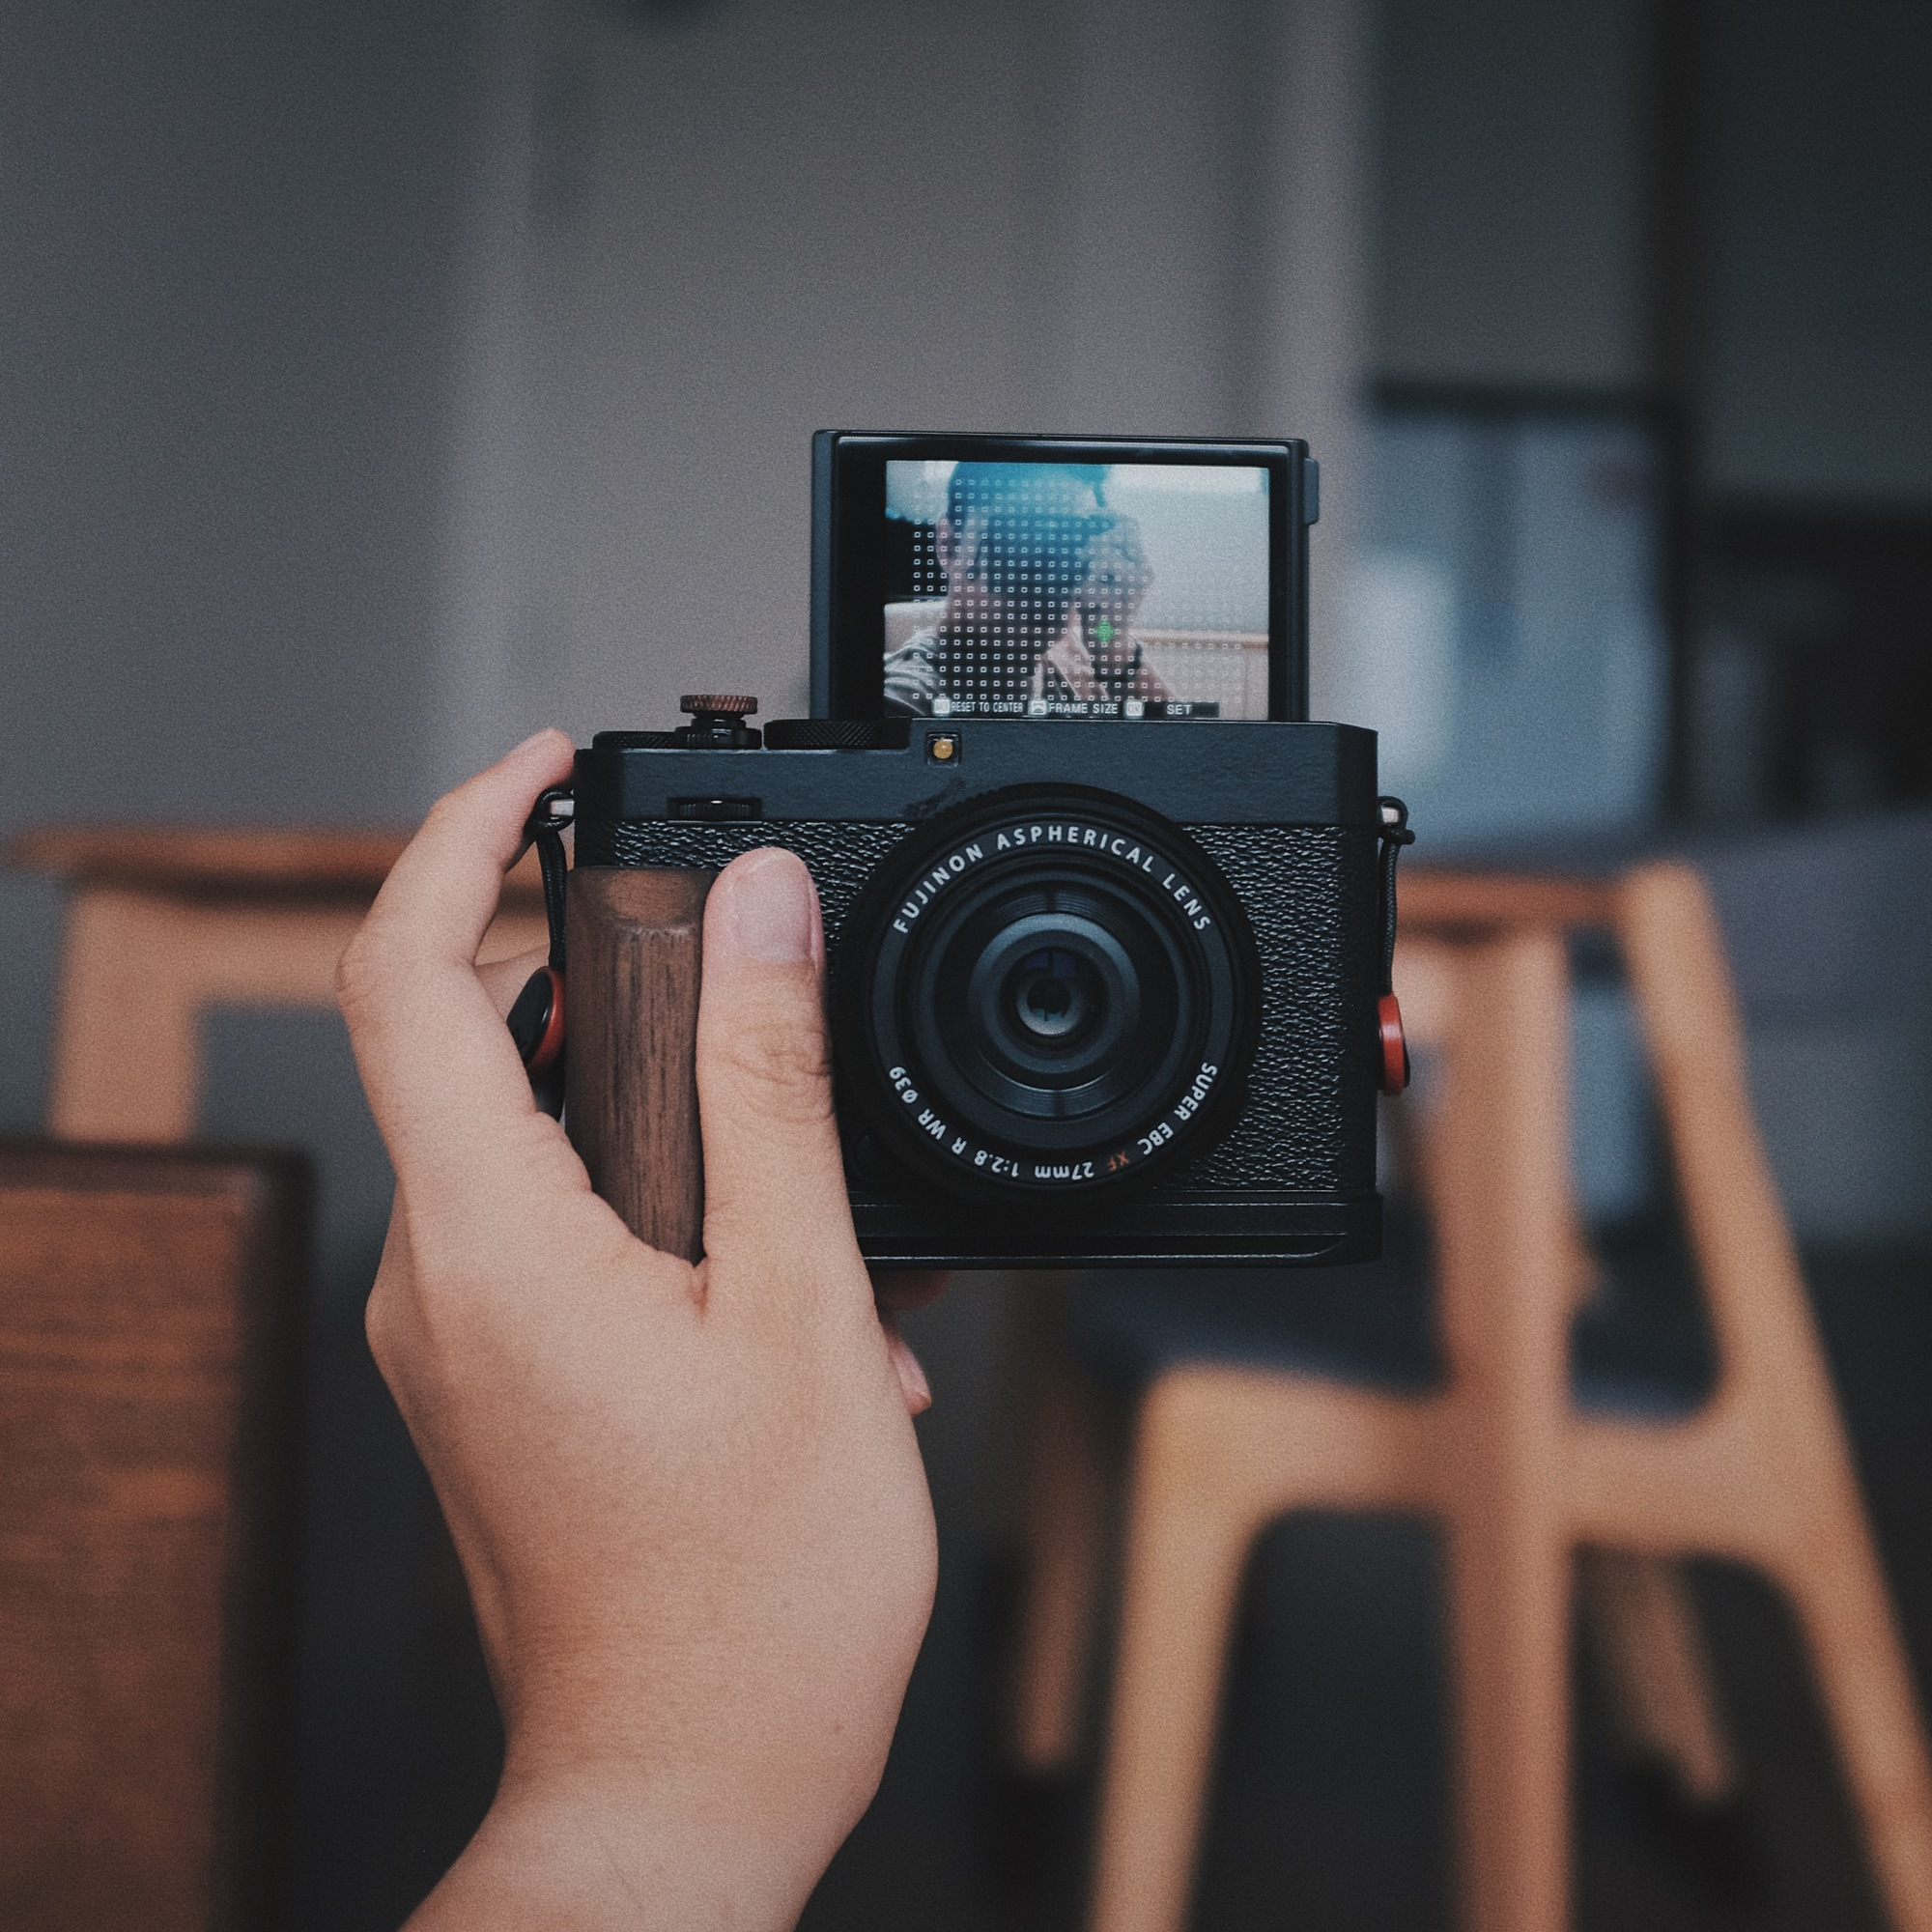
\includegraphics[width=\linewidth]{\envfinaldir/coverpic-prod.jpg}\par
            % \vskip 30pt
            \vfill

            \normalsize\rmfamily\scshape
            \copyright{} The Web Digest Project \hfill\large \envdatestr
        \end{center}
    \end{titlepage}
    % \restoregeometry
}
\newcommand{\simplehref}[1]{%
    \textcolor{blue!80!green}{\href{#1}{#1}}%
}
\renewcommand{\contentsname}{\center\Huge\sffamily\bfseries Contents\par\vskip 20pt}
\newcounter{ipartcounter}
\setcounter{ipartcounter}{0}
\newcommand{\ipart}[1]{
    % \vskip 20pt
    \clearpage
    \stepcounter{ipartcounter}
    \phantomsection
    \addcontentsline{toc}{chapter}{#1}
    % \begin{center}
    %     \Huge
    %     \sffamily\bfseries
    %     #1
    % \end{center}
    % \vskip 20pt plus 7pt
}
\newcounter{ichaptercounter}
\setcounter{ichaptercounter}{0}
\newcommand{\ichapter}[1]{
    % \vskip 20pt
    \clearpage
    \stepcounter{ichaptercounter}
    \phantomsection
    \addcontentsline{toc}{section}{\numberline{\arabic{ichaptercounter}}#1}
    \begin{center}
        \Huge
        \sffamily\bfseries
        #1
    \end{center}
    \vskip 20pt plus 7pt
}
\newcommand{\entrytitlefont}[1]{\subsection*{\raggedright\Large\sffamily\bfseries#1}}
\newcommand{\entryitemGeneric}[2]{
    % argv: title, url
    \parbox{\linewidth}{
        \entrytitlefont{#1}\par\vskip 5pt
        \footnotesize\ttfamily\mdseries
        \simplehref{#2}
    }\vskip 11pt plus 11pt minus 1pt
}
\newcommand{\entryitemGithub}[3]{
    % argv: title, url, desc
    \parbox{\linewidth}{
        \entrytitlefont{#1}\par\vskip 5pt
        \footnotesize\ttfamily\mdseries
        \simplehref{#2}\par\vskip 5pt
        \small\rmfamily\mdseries#3
    }\vskip 11pt plus 11pt minus 1pt
}
\newcommand{\entryitemAp}[3]{
    % argv: title, url, desc
    \parbox{\linewidth}{
        \entrytitlefont{#1}\par\vskip 5pt
        \footnotesize\ttfamily\mdseries
        \simplehref{#2}\par\vskip 5pt
        \small\rmfamily\mdseries#3
    }\vskip 11pt plus 11pt minus 1pt
}
\newcommand{\entryitemHackernews}[3]{
    % argv: title, hnurl, rawurl
    % \parbox{\linewidth}{
    %     \entrytitlefont{#1}\par\vskip 5pt
    %     \footnotesize\ttfamily\mdseries
    %     \simplehref{#3}\par
    %     \textcolor{black!50}{\href{#2}{#2}}
    % }\vskip 11pt plus 11pt minus 1pt
    \begin{minipage}{\linewidth}
            \entrytitlefont{#1}\par\vskip 5pt
            \footnotesize\ttfamily\mdseries
            \simplehref{#3}\par
            \textcolor{black!50}{\href{#2}{#2}}
    \end{minipage}\par\vskip 11pt plus 11pt minus 1pt
}







\begin{document}

\makeheader

\tableofcontents\clearpage




\ipart{Developers}
\ichapter{Hacker News}
\entryitemTwoLinks{DOJ will push Google to sell off Chrome}{https://news.ycombinator.com/item?id=42177767}{https://www.bloomberg.com/news/articles/2024-11-18/doj-will-push-google-to-sell-off-chrome-to-break-search-monopoly}

\entryitemTwoLinks{Finland and Lithuania Report Severed Undersea Data Cables}{https://news.ycombinator.com/item?id=42175676}{https://www.bloomberg.com/news/articles/2024-11-18/finland-says-subsea-germany-link-serving-data-centers-is-severed}

\entryitemTwoLinks{AMD now has more compute on the top 500 than Nvidia}{https://news.ycombinator.com/item?id=42175624}{https://www.nextplatform.com/2024/11/18/amd-now-has-more-compute-on-the-top500-than-nvidia/}

\entryitemTwoLinks{Fun facts about Google Scholar}{https://news.ycombinator.com/item?id=42175023}{https://blog.google/outreach-initiatives/education/google-scholar-20-years/}

\entryitemTwoLinks{Unreal 5.5 is a big deal [video]}{https://news.ycombinator.com/item?id=42174840}{https://www.youtube.com/watch?v=BcmUZpdChhA}

\entryitemTwoLinks{Show HN: FastGraphRAG – Better RAG using good old PageRank}{https://news.ycombinator.com/item?id=42174829}{https://github.com/circlemind-ai/fast-graphrag}

\entryitemTwoLinks{MailCatcher runs a super simple SMTP server}{https://news.ycombinator.com/item?id=42174231}{https://mailcatcher.me/}

\entryitemTwoLinks{Launch HN: Regatta Storage (YC F24) – Turn S3 into a local-like, POSIX cloud FS}{https://news.ycombinator.com/item?id=42174204}{https://news.ycombinator.com/item?id=42174204}

\entryitemTwoLinks{A BBC navigation bar component broke depending on the external monitor}{https://news.ycombinator.com/item?id=42173233}{https://www.joshtumath.uk/posts/2024-11-08-how-a-bbc-navigation-bar-component-broke-depending-on-which-external-monitor-it-was-on/}

\entryitemTwoLinks{Show HN: Tips.io – A Tailwind playground with AI, page management, and theming}{https://news.ycombinator.com/item?id=42173119}{https://tips.io}

\entryitemTwoLinks{The Skyline algorithm for packing 2D rectangles}{https://news.ycombinator.com/item?id=42173114}{https://jvernay.fr/en/blog/skyline-2d-packer/implementation/}

\entryitemTwoLinks{Bhutan, after prioritizing happiness, now faces an existential crisis}{https://news.ycombinator.com/item?id=42172281}{https://www.cbsnews.com/news/bhutan-emigration-crisis-60-minutes/}

\entryitemTwoLinks{Show HN: Documind – Open-source AI tool to turn documents into structured data}{https://news.ycombinator.com/item?id=42171311}{https://github.com/DocumindHQ/documind}

\entryitemTwoLinks{I was banned from the hCaptcha accessibility account for not being blind (2023)}{https://news.ycombinator.com/item?id=42171164}{https://michaels.world/2023/11/i-was-banned-from-the-hcaptcha-accessibility-account-for-not-being-blind/}

\entryitemTwoLinks{LLaVA-O1: Let Vision Language Models Reason Step-by-Step}{https://news.ycombinator.com/item?id=42171043}{https://arxiv.org/abs/2411.10440}

\entryitemTwoLinks{Reactive HTML Notebooks}{https://news.ycombinator.com/item?id=42170740}{https://maxbo.me/a-html-file-is-all-you-need.html}

\entryitemTwoLinks{Against Best Practices}{https://news.ycombinator.com/item?id=42170552}{https://www.arp242.net/best-practices.html}

\entryitemTwoLinks{We are shutting down Ondsel}{https://news.ycombinator.com/item?id=42169998}{https://ondsel.com/blog/goodbye/}

\entryitemTwoLinks{How Japanese black companies oppress workers (2014)}{https://news.ycombinator.com/item?id=42169615}{https://www.tofugu.com/japan/japanese-black-companies/}

\entryitemTwoLinks{Linux kernel 6.12 has been released}{https://news.ycombinator.com/item?id=42169418}{https://lwn.net/Articles/997958/}\ichapter{Phoronix}
\entryitemGeneric{\hskip 0pt{}AMD Begins Adding "GFX950" GPU Support To LLVM For Next CDNA Accelerator}{https://www.phoronix.com/news/AMD-GFX950-LLVM-Start}

\entryitemGeneric{\hskip 0pt{}Linux 6.13 Quadrupling Workqueue Concurrency Limit}{https://www.phoronix.com/news/Linux-6.13-Workqueues}

\entryitemGeneric{\hskip 0pt{}Ubuntu Praises 5~7\% PGO Compiler Optimization Performance Benefits}{https://www.phoronix.com/news/Ubuntu-PGO-Praises-Performance}

\entryitemGeneric{\hskip 0pt{}Linux 6.13 Rolling Out NVMe 2.1 Support \& NVMe Rotational Media}{https://www.phoronix.com/news/Linux-6.13-Block-NVMe}

\entryitemGeneric{\hskip 0pt{}New AMD ERAPS Feature Yields Additional Performance Gains On Zen 5}{https://www.phoronix.com/review/amd-zen5-eraps}

\entryitemGeneric{\hskip 0pt{}GCC 15 Compiler Development Shifts From Features To Bug Fixing}{https://www.phoronix.com/news/GCC-15-Enters-Stage-3}

\entryitemGeneric{\hskip 0pt{}Raspberry Pi OS Now Defaults To 512MB Swap, Updates Labwc Compositor}{https://www.phoronix.com/news/Raspberry-Pi-OS-Nov-2024}

\entryitemGeneric{\hskip 0pt{}LLVM Clang 20 Merges Intel Diamond Rapids Support With "-march=diamondrapids"}{https://www.phoronix.com/news/LLVM-Clang-20-Diamond-Rapids}

\entryitemGeneric{\hskip 0pt{}DXVK 2.5.1 Released To Fix A Major Regression \& Other Bugs}{https://www.phoronix.com/news/DXVK-2.5.1-Released}


\ipart{Developers~~~~(zh-Hans)}
\ichapter{Solidot}
\entryitemGeneric{\hskip 0pt{}空气污染与湿疹存在相关性}{https://www.solidot.org/story?sid=79807}

\entryitemGeneric{\hskip 0pt{}中国在珠海航展上展示可重复使用的昊龙货运航天飞机}{https://www.solidot.org/story?sid=79806}

\entryitemGeneric{\hskip 0pt{}微软释出 Windows 11 for Arm 镜像下载}{https://www.solidot.org/story?sid=79805}

\entryitemGeneric{\hskip 0pt{}研究发现 X 算法偏爱共和党和马斯克}{https://www.solidot.org/story?sid=79804}

\entryitemGeneric{\hskip 0pt{}美国四分之三的成年人超重或肥胖}{https://www.solidot.org/story?sid=79803}

\entryitemGeneric{\hskip 0pt{}OpenWrt 将改用 apk 包管理器}{https://www.solidot.org/story?sid=79802}

\entryitemGeneric{\hskip 0pt{}库克使用罗技的鼠标}{https://www.solidot.org/story?sid=79801}

\entryitemGeneric{\hskip 0pt{}Linux 6.12 释出}{https://www.solidot.org/story?sid=79800}

\entryitemGeneric{\hskip 0pt{}巴基斯坦宗教机构称使用 VPN 违反了伊斯兰教法}{https://www.solidot.org/story?sid=79799}

\entryitemGeneric{\hskip 0pt{}Google AI 聊天机器人建议人类去死}{https://www.solidot.org/story?sid=79798}

\entryitemGeneric{\hskip 0pt{}BASIC 语言合作者 Thomas Kurtz 去世}{https://www.solidot.org/story?sid=79797}

\entryitemGeneric{\hskip 0pt{}互联网档案馆提供《虚幻》和《虚幻竞技场》的免费下载}{https://www.solidot.org/story?sid=79796}

\entryitemGeneric{\hskip 0pt{}微重力下的精子活性显著下降}{https://www.solidot.org/story?sid=79795}

\entryitemGeneric{\hskip 0pt{}全世界的糖尿病患者人数超过了 8 亿}{https://www.solidot.org/story?sid=79794}

\entryitemGeneric{\hskip 0pt{}NSO Group 而不是政府客户运营着间谍软件}{https://www.solidot.org/story?sid=79793}

\entryitemGeneric{\hskip 0pt{}Valve 庆祝《半条命2》二十周年,游戏限时免费}{https://www.solidot.org/story?sid=79792}

\entryitemGeneric{\hskip 0pt{}Yandex 禁止中国 IP 搜索图片和视频}{https://www.solidot.org/story?sid=79791}\ichapter{V2EX}
\entryitemGeneric{\hskip 0pt{}[App Store] 续集: Apple Review Team 带着小姨子出现了}{https://www.v2ex.com/t/1090677}

\entryitemGeneric{\hskip 0pt{}[推广] Giffgaff eSIM 激活码免费发放(长期) - ⛄2024 冬季版}{https://www.v2ex.com/t/1090676}

\entryitemGeneric{\hskip 0pt{}[问与答] 求推荐一个医疗保险}{https://www.v2ex.com/t/1090675}

\entryitemGeneric{\hskip 0pt{}[分享创造] 在线生成: Barbie Font}{https://www.v2ex.com/t/1090674}

\entryitemGeneric{\hskip 0pt{}[机械键盘] 请教定制键盘}{https://www.v2ex.com/t/1090673}

\entryitemGeneric{\hskip 0pt{}[Apple] 请愿小米为 Mac mini 出一款 24 寸 4K 显示器}{https://www.v2ex.com/t/1090672}

\entryitemGeneric{\hskip 0pt{}[iOS] 刚买一年的手机被偷了,想从安卓转到苹果试试}{https://www.v2ex.com/t/1090671}

\entryitemGeneric{\hskip 0pt{}[分享创造] windsurf 资料整理}{https://www.v2ex.com/t/1090670}

\entryitemGeneric{\hskip 0pt{}[Google] Google Maps 帮助德国餐馆删差评}{https://www.v2ex.com/t/1090669}

\entryitemGeneric{\hskip 0pt{}[问与答] microsoft copilot 突然用不了了, 9 月份还可以。现在开全局代理,报如下错误: 无法访问此网站 copilot.microsoft.com 意外终止了连接。  持续一周了,求解决}{https://www.v2ex.com/t/1090668}

\entryitemGeneric{\hskip 0pt{}[问与答] 网站被百度收录了,但是搜狗和 360 未收录}{https://www.v2ex.com/t/1090667}

\entryitemGeneric{\hskip 0pt{}[职场话题] 社招的移动客户端面试中考查算法题的比重大吗}{https://www.v2ex.com/t/1090666}

\entryitemGeneric{\hskip 0pt{}[问与答] 有什么移动电源可以用在 macmini 上并且可以上飞机}{https://www.v2ex.com/t/1090665}

\entryitemGeneric{\hskip 0pt{}[问与答] 工作中遇到把别人工作说成自己产出的人,该怎么办}{https://www.v2ex.com/t/1090664}

\entryitemGeneric{\hskip 0pt{}[生活] 突然感受到一年级那堂作文课对我这些年的影响}{https://www.v2ex.com/t/1090663}

\entryitemGeneric{\hskip 0pt{}[硬件] N100 小主机,使用路由器 UPS 保障断电,有何办法让小主机``感知''AC 已经断电、还有电池快耗尽呢?}{https://www.v2ex.com/t/1090662}

\entryitemGeneric{\hskip 0pt{}[Apple] apple music 国区家庭会员车}{https://www.v2ex.com/t/1090660}

\entryitemGeneric{\hskip 0pt{}[分享创造] 🥳 我给 imgfans 图床写了个 Chrome 扩展,求测试呀!}{https://www.v2ex.com/t/1090658}

\entryitemGeneric{\hskip 0pt{}[Apple] 日版 iPhone 收到后准备下载 ultra APP 转 ESIM,结果让我短信验证,咋办}{https://www.v2ex.com/t/1090657}

\entryitemGeneric{\hskip 0pt{}[问与答] 外包公司外包人员是替罪羊吗}{https://www.v2ex.com/t/1090656}

\entryitemGeneric{\hskip 0pt{}[问与答] 客户可以物理接触到电脑,有什么办法保证电脑上程序不被拷贝走。windows,硬件是 amd 8700g}{https://www.v2ex.com/t/1090655}

\entryitemGeneric{\hskip 0pt{}[数据库] MySQL 支持跨库事务吗?}{https://www.v2ex.com/t/1090654}

\entryitemGeneric{\hskip 0pt{}[Apple] macOS 15, windows 官方开发的远程桌面工具,我为啥每次连接都是显示凭据错误,远程桌面到底应该怎么用}{https://www.v2ex.com/t/1090653}

\entryitemGeneric{\hskip 0pt{}[问与答] 有关 GRUB 美化的一些小问题:它没有给某些启动项分配图标,怎么手动调用?}{https://www.v2ex.com/t/1090652}

\entryitemGeneric{\hskip 0pt{}[问与答] 只有我觉得 windows 办公效率比 macbook 强吗?}{https://www.v2ex.com/t/1090651}

\entryitemGeneric{\hskip 0pt{}[宽带症候群] 有办法测试出拨号宽带的并发连接数吗?}{https://www.v2ex.com/t/1090648}

\entryitemGeneric{\hskip 0pt{}[酷工作] [远程] 急招测试工程师}{https://www.v2ex.com/t/1090647}

\entryitemGeneric{\hskip 0pt{}[Apple] 每次 iOS 更新都会导致 Siri 的一些实用指令失灵}{https://www.v2ex.com/t/1090645}

\entryitemGeneric{\hskip 0pt{}[问与答] 目前最好用的文字生成 logo 的工具还是 Midjourney 么?}{https://www.v2ex.com/t/1090644}

\entryitemGeneric{\hskip 0pt{}[分享创造] initx 一个 Node.js 脚本引擎}{https://www.v2ex.com/t/1090643}

\entryitemGeneric{\hskip 0pt{}[macOS] 发现了 Mac 桌面歌词软件 LyricsX 的个人维护版}{https://www.v2ex.com/t/1090642}

\entryitemGeneric{\hskip 0pt{}[问与答] 如何运营一个 job board 呢?}{https://www.v2ex.com/t/1090641}

\entryitemGeneric{\hskip 0pt{}[问与答] 隔壁在收 v 站邀请, 100 个批发}{https://www.v2ex.com/t/1090640}

\entryitemGeneric{\hskip 0pt{}[问与答] M1 系列 MacBook pro 有什么办法可以大幅度提升续航?  充电宝放上去 30w 好像 1w 毫安也充不了多少、 设置为外部供电模式不给电池充电的情况 也掉的很快}{https://www.v2ex.com/t/1090639}

\entryitemGeneric{\hskip 0pt{}[Apple] 奇葩,油管要求更新尼区付款却成功扣款}{https://www.v2ex.com/t/1090638}

\entryitemGeneric{\hskip 0pt{}[问与答] iOS 上面浏览器可以正常进入奈飞并观看。换成 iOS 奈飞客户端 就不能登陆观看了。这是什么情况呀。}{https://www.v2ex.com/t/1090637}

\entryitemGeneric{\hskip 0pt{}[问与答] [推广]软考刷题神器,想软考的朋友有福了}{https://www.v2ex.com/t/1090635}

\entryitemGeneric{\hskip 0pt{}[OpenAI] ChatGPT 的 Windows 客户端如何在 Edge 浏览器启用 Proxy SwitchyOmega 扩展的情况下也能正常让其内置 WebView 组件正常联网登录 OpenAI 账号?}{https://www.v2ex.com/t/1090634}

\entryitemGeneric{\hskip 0pt{}[问与答] 单房间 50 平方,有没有推荐的电取暖器?还是需要买两个才能支持?}{https://www.v2ex.com/t/1090633}

\entryitemGeneric{\hskip 0pt{}[Apple] macOS 的``媒体与购买项目''不可以单独登录吗}{https://www.v2ex.com/t/1090632}

\entryitemGeneric{\hskip 0pt{}[问与答] 我看到有些国外服务(比如 Vultr)支持支付宝跨币种结算,他们是怎么做到的?}{https://www.v2ex.com/t/1090631}

\entryitemGeneric{\hskip 0pt{}[分享发现] Play Sprunki Retake online}{https://www.v2ex.com/t/1090630}

\entryitemGeneric{\hskip 0pt{}[分享发现] 分享一下我博客的图床思路: Git Hook + Python 图片转 WebP}{https://www.v2ex.com/t/1090629}

\entryitemGeneric{\hskip 0pt{}[问与答] Mysql 中 TinyInt 和 Java 中的 bool 对象转换问题}{https://www.v2ex.com/t/1090628}

\entryitemGeneric{\hskip 0pt{}[问与答] kvm 这玩意有讲究吗?想买个切换 Windows PC 和 mac mini}{https://www.v2ex.com/t/1090626}

\entryitemGeneric{\hskip 0pt{}[OpenWrt] 有啥便宜的带 Wi-Fi 的 openwrt 软路由推荐吗?}{https://www.v2ex.com/t/1090625}

\entryitemGeneric{\hskip 0pt{}[分享发现] 又一个 newsletter}{https://www.v2ex.com/t/1090623}

\entryitemGeneric{\hskip 0pt{}[分享创造] 什么?!犄角旮旯 Wi-Fi 路由器信号总是若有若无?这个工具或许可以帮到你!}{https://www.v2ex.com/t/1090622}

\entryitemGeneric{\hskip 0pt{}[问与答] 饿了么优惠券}{https://www.v2ex.com/t/1090621}

\entryitemGeneric{\hskip 0pt{}[程序员] Typora 通过文件夹管理 md 文件时,本地图片该怎么链接?}{https://www.v2ex.com/t/1090620}


\ipart{Generic News}
\ichapter{AP News}
\entryitemWithDescription{\hskip 0pt{}MSNBC `Morning Joe' hosts say they met with Trump to reopen lines of communication}{https://apnews.com/article/cf4816dd28372a4c942d256df2e440ae}{}

\entryitemWithDescription{\hskip 0pt{}Beyoncé will perform at halftime of Ravens-Texans Christmas Day game on Netflix}{https://apnews.com/article/dcf2c5fb87a78cdc70e0cfc2f2683446}{}

\entryitemWithDescription{\hskip 0pt{}Actors Jonathan Majors and Meagan Good are engaged. She backed him through domestic violence trial}{https://apnews.com/article/715c7ffbf1686956445923078d80014a}{}

\entryitemWithDescription{\hskip 0pt{}Suzuki and Sabathia among 14 newcomers on baseball Hall of Fame ballot. Wagner tops holdovers}{https://apnews.com/article/b962ec5705d47ce011ae7b4e1228749b}{}

\entryitemWithDescription{\hskip 0pt{}Sean `Diddy' Combs lawyers claim seizure of writings from cell is `outrageous government conduct'}{https://apnews.com/article/c3d870409248192e82306162170b6da7}{}

\entryitemWithDescription{\hskip 0pt{}WWE's `Monday Night Raw' on Netflix will debut on Jan. 6 in Los Angeles}{https://apnews.com/article/a7b7aa16c1c061930acb8262e5bc1f02}{}

\entryitemWithDescription{\hskip 0pt{}Herlda Senhouse, the second-oldest U.S. resident, dies at age 113}{https://apnews.com/article/4224e9f97431f88c82b92a280d37f464}{}

\entryitemWithDescription{\hskip 0pt{}Indigenous senator who yelled `You are not our king' at Charles III is censured in Australia}{https://apnews.com/article/2b8d6ce8bcaa14ee5fe10a719a7790d0}{}

\entryitemWithDescription{\hskip 0pt{}About 20\% of Americans regularly get their news from influencers on social media, report says}{https://apnews.com/article/eacd42bce73d6e11cbc760caf28c993a}{}

\entryitemWithDescription{\hskip 0pt{}Raiders' Brock Bowers and other NFL players celebrate TDs with Trump-inspired dance moves}{https://apnews.com/article/013fa86a963809b4b6d87e0c4774de13}{}

\entryitemWithDescription{\hskip 0pt{}Josh Allen seals Bills' 30-21 win over Chiefs with TD run, ending bid for perfect season}{https://apnews.com/article/9d2b3c026b22b11ed5a881e97c0e404a}{}

\entryitemWithDescription{\hskip 0pt{}Hollywood stars gather for honorary Oscars event celebrating Quincy Jones, Bond producers, more}{https://apnews.com/article/bbd0d5811502a5d907e0f405a9736a51}{}

\entryitemWithDescription{\hskip 0pt{}Veteran news executive Reg Murphy, who survived abduction decades ago, has died at 90}{https://apnews.com/article/91d409971a3db9c0906b843e684a8742}{}\ichapter{Reuters}
\entryitemWithDescription{\hskip 0pt{}North American leaders talk cooperation on G20 sidelines}{https://www.reuters.com/world/americas/north-american-leaders-talk-cooperation-g20-sidelines-2024-11-18/}{Mexican President Claudia Sheinbaum spoke with both outgoing U.S. President Joe Biden as well as Canadian Prime Minister Justin Trudeau on the sidelines of the G20 summit in Brazil on...}

\entryitemWithDescription{\hskip 0pt{}US says Russia escalated Ukraine conflict by deploying North Koreans}{https://www.reuters.com/world/us-says-russia-escalated-ukraine-conflict-by-deploying-north-koreans-2024-11-18/}{The United States said on Monday it was Russia that is escalating the conflict in Ukraine by deploying North Korean troops, after the Kremlin warned that Washington would deepen its involvement in the war by allowing Kyiv\textquotesingle...}

\entryitemWithDescription{\hskip 0pt{}UN food agency to restart Haiti aid flights after planes hit by gunfire}{https://www.reuters.com/world/americas/un-food-agency-restart-haiti-aid-flights-after-planes-hit-by-gunfire-2024-11-18/}{The United Nations Humanitarian Air Service will restart food aid flights to Haiti on Wednesday after around a week\textquotesingle s hiatus and resolving regulatory issues, according to a statement from the U.N. World Food Programme...}

\entryitemWithDescription{\hskip 0pt{}US warns Turkey against hosting Hamas leaders}{https://www.reuters.com/world/us-warns-turkey-against-hosting-hamas-leaders-2024-11-18/}{The United States warned Turkey on Monday against hosting Hamas leadership, saying Washington does not believe leaders of a terrorist organization should be living...}

\entryitemWithDescription{\hskip 0pt{}US Sudan envoy meets army chief Burhan on first visit}{https://www.reuters.com/world/africa/us-sudan-envoy-meets-army-chief-burhan-first-visit-2024-11-18/}{The U.S. special envoy to Sudan travelled to the African country for the first time on Monday to seek an increase in the flow of aid to millions of people in need and an end to a devastating...}

\entryitemWithDescription{\hskip 0pt{}U.S. Senate to consider measures blocking some weapons sales to Israel}{https://www.reuters.com/world/us-senate-consider-measures-blocking-some-weapons-sales-israel-2024-11-18/}{The Senate could vote as soon as Wednesday on legislation to block arms sales to...}

\entryitemWithDescription{\hskip 0pt{}Lebanon submits written response to U.S. truce proposal, Lebanese official and local media say}{https://www.reuters.com/world/lebanon-submits-written-response-us-truce-proposal-lebanese-official-local-media-2024-11-18/}{Lebanon has submitted a written response to a U.S. truce proposal, a Lebanese official source and Lebanese broadcaster Al-Jadeed said on...}

\entryitemWithDescription{\hskip 0pt{}Woman killed by rocket attack in northern Israel, medics say}{https://www.reuters.com/world/middle-east/woman-killed-by-rocket-attack-northern-israel-medics-say-2024-11-18/}{A woman was killed and several other people were wounded on Monday when a rocket struck a building in a northern Israeli town, Israel\textquotesingle s ambulance service...}

\entryitemWithDescription{\hskip 0pt{}Eleven people arrested after explosion, fire at gas complex, Venezuela minister says}{https://www.reuters.com/world/americas/eleven-people-arrested-after-explosion-fire-gas-complex-venezuela-minister-says-2024-11-18/}{Eleven people have been arrested as part of an investigation into an explosion and fire at a major gas complex last week, Venezuela\textquotesingle s vice-president and oil minister Delcy Rodriguez said on...}

\entryitemWithDescription{\hskip 0pt{}NZ Maori protest march reaches Wellington for rally against Indigenous bill}{https://www.reuters.com/world/asia-pacific/nz-maori-protest-march-reaches-wellington-rally-against-indigenous-bill-2024-11-18/}{A nine-day march by Maori and their supporters across New Zealand will culminate in Wellington on Tuesday at a rally where thousands are expected to protest a bill that opponents say seeks to dilute the rights of the...}

\entryitemWithDescription{\hskip 0pt{}Members of UN Security Council call for surge in assistance to Gaza}{https://www.reuters.com/world/members-un-security-council-call-surge-assistance-gaza-2024-11-18/}{Members of the United Nations Security Council called on Monday for a surge in assistance to reach people in need in Israeli-basieged Gaza, warning that the situation in the Palestinian enclave was getting...}

\entryitemWithDescription{\hskip 0pt{}Netanyahu says Israel's October attack hit a component in Iran nuclear programme}{https://www.reuters.com/business/aerospace-defense/netanyahu-says-israels-october-attack-hit-component-iran-nuclear-programme-2024-11-18/}{Prime Minister Benjamin Netanyahu said on Monday that Israel\textquotesingle s air attack on Iran last month hit an element of Tehran\textquotesingle s nuclear programme while degrading its defence and missile production...}

\entryitemWithDescription{\hskip 0pt{}Backers of Argentina's Milei launch 'armed' group to support far-right president}{https://www.reuters.com/world/americas/backers-argentinas-milei-launch-armed-group-support-far-right-president-2024-11-18/}{A group of supporters of Argentine President Javier Milei announced the creation of what they termed an armed wing of his libertarian party, touting the group as loyal foot soldiers determined to defend the far-right politician...}\ichapter{联合早报}
\entryitemWithDescription{沈泽玮:台湾冲突阻遏法案只叫不咬?}{https://www.zaobao.com/news/china/story20240918-4758889}{美国众议院9月9日开启了长达一星期的``中国周'',共通过25项主要涉华法案。(法新社) 美国众议院在当地时间9月9日开启了长达一星期的``中国周'',在美国总统和国会选举举行之前,密集表决数十项与中国有关的法案,共通过25项主要涉华法案……}

\entryitemWithDescription{欧盟电动车关税投票倒计时 中国在分歧中寻支持}{https://www.zaobao.com/news/china/story20240917-4758953}{欧盟27个成员国将于9月25日就是否继续对进口自中国的电动汽车额外征税进行最后表决。图为上海港等待装运出口的电动汽车。(彭博社) 欧盟对中国电动汽车加征关税的投票进入倒计时,正在欧洲访问的中国商务部部长王文涛与欧盟多国政府高层就此进行协商,试图在立场分歧的成员国中争取到更多支持。 受访学者研判,欧盟对中国电动汽车加征关税不可避免,但具体的加税方式和幅度仍有一定弹性,这是王文涛此行与各国谈判的重点……}

\entryitemWithDescription{港府今年将举办逾400项国庆活动}{https://www.zaobao.com/news/china/story20240917-4759341}{再过十多天就是中国国庆75周年,香港天星小轮展示``国庆75周年''\,``三天免费搭小轮''等标语迎国庆。(中新社) 再过十多天就是中国国庆75周年,香港特区政府今年将举办逾400项庆祝活动,希望通过一连串活动庆祝国庆,并且弘扬爱国主义教育及刺激消费。 港府星期二(9月17日)召开记者会,介绍各项庆祝国庆活动和特别优惠,涉及出行及吃喝玩乐等领域……}

\entryitemWithDescription{美空军部长:中国大陆军演精密化 为入侵封锁台湾做准备}{https://www.zaobao.com/news/china/story20240917-4759407}{美国空军部长肯德尔星期一(9月16日)在空军暨太空军协会的一场大会上致辞,提到中国对印太地区日益增长的威胁。(取自美国国防部网站) (华盛顿综合讯)美国空军部长肯德尔指,中国大陆军演的规模越来越大,也更加精密化,这是在专门为入侵、封锁台湾做准备。他也称,中国对印太地区的威胁现在已存在……}

\entryitemWithDescription{批准潜在对台备件军售案后 美派巡逻机过航台海}{https://www.zaobao.com/news/china/story20240917-4758770}{台军士兵8月26日在屏东县枋山训练场进行实弹演习时,从M1167 TOW运载车上发射一枚美制TOW-2A线导反坦克导弹。(路透社) (华盛顿/台北/北京综合讯)在批准潜在对台备件军售案之后,美国派遣反潜巡逻机过航台湾海峡,中国人民解放军东部战区则组织战机跟监美机,并誓言``坚决捍卫国家主权''……}

\entryitemWithDescription{李家超:若香港驻美经贸办被关 受害的是美企}{https://www.zaobao.com/news/china/story20240917-4758797}{香港特首李家超星期一(9月17日)警告,如果美国通过法案,导致香港驻美经贸办关闭,受害的是美国企业。图为李家超9月11日在``一带一路''高峰论坛上致辞。(彭博社) (香港综合讯)香港特首李家超警告,如果美国通过法案,导致香港驻美经贸办关闭,受害的是美国企业。 美国众议院上周通过《香港经济贸易办事处认证法案》,如果参议院也表决通过并交由总统签署成法,香港三个驻美国的经贸办可能将被强制关闭……}

\entryitemWithDescription{美国指中国航空工业集团员工企图实施黑客攻击}{https://www.zaobao.com/news/china/story20240917-4757988}{(华盛顿综合讯)中国航空航天巨头中国航空工业集团一名员工被指试图对美国宇航局、美国军方和其他目标展开黑客攻击。 据彭博社报道,美国检察官布坎南星期一(9月16日)在起诉书中,指控中国航空工业集团39岁的工程师吴宋(音译,Song Wu)企图从美国宇航局、空军、陆军和海军,以及联邦航空管理局取得电脑软件和源代码……}

\entryitemWithDescription{【东谈西论】恒大账务造假 普华永道是共犯还是被拖累?}{https://www.zaobao.com/news/china/story20240917-4756452}{因涉及恒大地产审计项目的违法行为,普华永道中国9月13日被中国财政部和证监会处以4.41亿人民币罚款并被令停业六个月, 广州分所被撤销……}

\entryitemWithDescription{戴庆成:香港输入人才计划大检阅}{https://www.zaobao.com/news/china/story20240917-4744978}{香港于2022年底推出高端人才通行证计划。(法新社) 2019年香港反修例风波过后,数以十万计港人移居海外,令香港出现人才荒。港府为了解决这个问题,在过去几年积极引入``新血'',当中以高才通计划最受瞩目,社会上也不时热议其成效。 高才通全称为高端人才通行证计划,于2022年底推出,申请人年收入须达到250万港元(约42万新元)以上,或本科毕业于全球百强大学并满足一定工作年限等……}

\entryitemWithDescription{中美希望稳定双边关系 中小国家可​​​搭建桥梁}{https://www.zaobao.com/news/china/story20240917-4745091}{中美元首去年11月在旧金山会晤后,双方都希望稳定两国关系,我国巡回大使陈庆珠认为,如果中美两国都认为走向战争不符合它们的利益,那么中小国家就可以做点什么,为双方搭建桥梁。 陈庆珠星期一(9月16日)在李光耀公共政策学院的一场研讨会上说,中国与西方的关系面对诸多困难,有中国智库表示,希望新加坡能协助在中美之间建立更多对话,``因为新加坡受美国信任,也在中国有渠道''……}

\entryitemWithDescription{陈庆珠:世界经历了三次``中国冲击'' 中美的主导力之争将继续}{https://www.zaobao.com/news/china/story20240917-4744996}{李光耀公共政策学院``思想之节庆''的一场研讨会,讨论``历史终结时的中国冲击''。左起是我国巡回大使陈庆珠、通商中国主席李奕贤、李光耀公共政策学院国际关系助理教授何莉菁、李光耀公共政策学院院长柯成兴……}

\entryitemWithDescription{上海遭遇75年来最强台风 扰乱民众中秋假期出行}{https://www.zaobao.com/news/china/story20240916-4745224}{台风贝碧嘉星期一(9月16日)登陆上海,维护人员星期一下午在衡山路上处理倒伏的树木。 (新华社) 台风造成上海上万株数目倒伏或折断。图为一棵倒下的大树砸坏一旁的建筑。(法新社) 台风贝碧嘉登陆上海后,黄浦江苏州河口潮位上涨,乌云密布。(中新社) 中国上海市星期一(9月16日)遭遇75年来最强台风``贝碧嘉''登陆,也是上海有记录以来首次有强台风侵袭……}

\entryitemWithDescription{陆男频长驱偷渡台湾在测试边防实力?}{https://www.zaobao.com/news/china/story20240916-4745161}{中国大陆一名王姓男子在中秋节前夕,乘橡皮艇从浙江宁波抵达台湾新北市林口,主动打电话投案,海巡署人员前去接他上岸。(自由時報) 中国大陆一名王姓男子划橡皮艇于上星期六清晨偷渡到台湾,隔天被新北市地方法院裁定羁押禁见。这是6月以来第二起大陆人士偷渡至台湾,此间专家质疑是否为海防破口,并怀疑对岸是否在测试台湾的边防实力……}

\entryitemWithDescription{中美时隔八月举行国防部工作会晤}{https://www.zaobao.com/news/china/story20240916-4745025}{(北京/华盛顿综合讯)中美双方上周末举行国防部工作会晤;美国官员称,美国积极进行美中两军外交活动,不代表美国对有关中国议题的处理方式发生任何改变。 据中国国防部星期天(15日)晚上通报,北京香山论坛结束后,第18次中美国防部工作会晤上星期六至星期天(9月14日至15日)在北京举行……}

\entryitemWithDescription{中国高校今年拟增足球运动本科专业}{https://www.zaobao.com/news/china/story20240916-4744925}{(北京综合讯)为了培养足球专业人才,中国大专学府今年度拟新增足球运动本科专业,以具体落实中国足球改革。 综合人民网和《南方都市报》报道,中国教育部上星期五(9月13日)发布《2024年度普通高等学校本科专业申报材料公示》。根据公示统计,今年度拟新增专业535个,涉及353所高校,其中39所高校新增足球运动专业……}

\entryitemWithDescription{香港23条首案 港男因穿``光时''上衣被定罪}{https://www.zaobao.com/news/china/story20240916-4743439}{(香港综合讯)香港一名无业男子,今年6月因穿印有2019年反修例抗争口号的上衣而被捕。他星期一承认违反煽动意图罪,成为在《维护国家安全条例》(即《香港基本法》第23条)下被定罪的第一人。 综合港媒《星岛日报》和路透社报道,27岁无业男子诸启邦今年6月12日在石门港铁站附近,未能出示身份证供查阅被警方拘捕……}

\entryitemWithDescription{美国务院:中国释放被关押近20年美籍牧师}{https://www.zaobao.com/news/china/story20240916-4744614}{(华盛顿综合电)中国释放被关押近20年的美国籍牧师,显示北京在中美关系的关键时刻展现善意。 综合彭博社、法新社和路透社报道,美国国务院发言人星期天(9月15日)说:``我们欢迎林大卫(音译,David Lin)从中华人民共和国的监狱获释。他已回返美国,这是他近20年来首次与家人见面。'' 林大卫的女儿艾丽斯告诉美国政治新闻网Politico,她的父亲将抵达得克萨斯州的圣安东尼奥……}

\entryitemWithDescription{中国驻泰使馆:近期并未向湄公河下游泄洪}{https://www.zaobao.com/news/china/story20240916-4743917}{(北京讯)泰国西北部的湄公河因洪水泛滥而决堤,中国否认这是中方泄洪所致,并称近来已持续减少云南景洪水电站的出库流量,以助下游地区抗洪。 中国驻泰国大使馆星期日(9月15日)深夜在官方微信公众号发文说,当天又有媒体报道称中国正在向湄公河泄洪,经向中国主管部门核实,使馆再次澄清,为帮助下游地区应对洪灾,中方近来持续稳定和减少景洪水电站出库流量,不可能对下游地区抗洪救灾形成压力……}

\entryitemWithDescription{加入美国储存可靠度评估计划 台湾军方编列预算采购三类型导弹}{https://www.zaobao.com/news/china/story20240916-4743826}{(台北讯)据台媒报道,台湾军方持续向美国采购可简易操作的导弹,预计在2024年、2031年以前获得400枚``标枪''反装甲导弹、2485枚``刺针''人携式防空导弹……}

\entryitemWithDescription{韩咏红:中美分头追逐全球南方}{https://www.zaobao.com/news/china/story20240916-4730719}{9月5日,中国外长王毅(中)同中非合作论坛非方现任共同主席国塞内加尔外长法勒(左)、下任共同主席国刚果外长加科索(右),在北京共同会见中外记者并答问。(路透社) 进入气候宜人的9月,中国接连举行了两场受瞩目的国际会议,一是聚集非洲53国国家元首与政要的中非合作论坛,接着是周末刚闭幕的北京香山论坛。 两场活动的参与者不同,规模也有很大差距……}

\entryitemWithDescription{菲律宾船只撤离中菲争议海域后 将再派船接替}{https://www.zaobao.com/news/china/story20240915-4730494}{这张在9月15日拍摄,并由菲律宾海岸警卫队提供的照片显示,菲律宾海岸警卫队船马格巴努亚号抵达了菲国巴拉望岛的一个港口。菲律宾早前以发现填海活动为由,今年4月派出马格巴努亚号前往萨比纳礁。(法新社/菲律宾海岸警卫队) 菲律宾国家海事委员会星期天(9月15日)发声明称,该国海岸警卫队一艘巡逻舰已离开萨比纳礁争议海域……}

\entryitemWithDescription{台风贝碧嘉直击中国华东 多趟本地与沪杭间航班取消}{https://www.zaobao.com/news/china/story20240915-4730611}{9月15日在上海外滩滨江步道上,一名外籍游客的雨伞被大风吹起。台风贝碧嘉的中心当天下午5时位于上海市东偏南方大约435公里的东海海面上,中心附近最大风力有13级。(中新社) (上海/新加坡综合讯)台风贝碧嘉预计将为中国华东沿海地区带来狂风暴雨,多趟往返新加坡与上海和杭州的航班取消……}






\clearpage
\leavevmode\vfill
\footnotesize

Copyright \copyright{} 2023-2024 Neruthes and other contributors.

This document is published with CC BY-NC-ND 4.0 license.

The entries listed in this newsletter may be copyrighted by their respective creators.

This newsletter is generated by the Web Digest project.

The newsletters are also delivered via Telegram channel \CJKunderline{\href{https://t.me/webdigestchannel}{https://t.me/webdigestchannel}}.\\
RSS feed is available at \CJKunderline{\href{https://webdigest.pages.dev/rss.xml}{https://webdigest.pages.dev/rss.xml}}.

This newsletter is available in PDF at
\CJKunderline{\href{https://webdigest.pages.dev/}{https://webdigest.pages.dev/}}.

The source code being used to generate this newsletter is available at\\
\CJKunderline{\href{https://github.com/neruthes/webdigest}{https://github.com/neruthes/webdigest}}.

This newsletter is also available in
\CJKunderline{\href{http://webdigest.pages.dev/readhtml/\envyear/WebDigest-20241119.html}{HTML}} and
\CJKunderline{\href{https://github.com/neruthes/webdigest/blob/master/markdown/\envyear/WebDigest-20241119.md}{Markdown}}.


\coverpic{https://unsplash.com/photos/a-view-of-a-mountain-range-with-trees-in-the-foreground-lYHT5fthhzM}{Jacob Grishey}


\end{document}
